\documentclass[12pt]{article}
\usepackage[utf8]{inputenc}
\usepackage[T2A]{fontenc}
\usepackage[russian]{babel}
\usepackage{amsmath}
\usepackage{amssymb}
\usepackage{dsfont}
\usepackage[dvipsnames]{xcolor}
\usepackage{setspace}
\usepackage{multirow}
\usepackage[a4paper, outer=1.5cm, inner=1.5cm, top=1cm, bottom=1cm]{geometry}
\usepackage{graphicx}
\usepackage{skull}
\usepackage{wasysym}
\usepackage{float}
\graphicspath{{.images/}}
\usepackage{hyperref}
\hypersetup{colorlinks=true, linkcolor=blue, filecolor=magenta, urlcolor=cyan}
\usepackage[firstpage]{draftwatermark}
\SetWatermarkText{
    $\qquad\qquad\qquad\qquad\qquad$\parbox{7cm}{\begin{center}
    
\includegraphics[width = 0.08\textwidth]{lion-logo.png}\bigskip\\~\bigskip\\~\vspace{-24mm}\\~\end{center}}
}
\SetWatermarkAngle{0}
\SetWatermarkScale{1.5}
\usepackage{etoolbox}

\newtoggle{ifsolved}
\newtoggle{needhelp}
\newcounter{num}
\setcounter{num}{1}

\newcommand{\newnum}{\par\textbf{\textnumero\arabic{num}}\stepcounter{num}}
\newcommand{\sol}{\vspace{3mm}\par\textbf{Решение: }}
\newcommand{\ans}{\vspace{3mm}\par\textbf{Ответ: }}
\newcommand{\hint}{\vspace{3mm}\par\textbf{Подсказка: }}
\newcommand{\mode}[1]{
\ifstrequal{#1}{0}{\togglefalse{ifsolved}\togglefalse{needhelp}}{\ifstrequal{#1}{1}{\togglefalse{ifsolved}\toggletrue{needhelp}}{\ifstrequal{#1}{2}{\toggletrue{ifsolved}\togglefalse{needhelp}}{\toggletrue{ifsolved}\toggletrue{needhelp}}}}} %if 0 - if 1 - if 2 - else
%\newenvironment{problem}[8]{%#1, #2, #3
%\parbox{\linewidth}{\vspace{4mm}\ifstrequal{#4}{(лёгкая)}{\newnum\textbf{.}}{\newnum\textbf{*.} } \\ #5}
%\iftoggle{ifsolved}{\sol #6}{}
%\iftoggle{ifsolved}{\ans #7}{}
%\iftoggle{needhelp}{\hint #8}{}}

\newenvironment{problem}[8]{%#1, #2, #3
\parbox{\linewidth}{\vspace{5mm}\ifstrequal{#4}{(лёгкая)}{\newnum\textbf{.}}{\newnum\textbf{*.} } \\ #5}
\iftoggle{ifsolved}{\sol #6}{}

\iftoggle{ifsolved}{\parbox{\linewidth}{\ans #7}}{}
\iftoggle{needhelp}{\parbox{\linewidth}{\hint #8}}{}}

\newenvironment{mylist} %custom list
{ \begin{itemize}
    \setlength{\itemsep}{0pt}
    \setlength{\parskip}{0pt}
    \setlength{\parsep}{0pt}     }
{ \end{itemize}                  }

\newenvironment{homeass}[1]{\vspace*{-1.5cm}
\iftoggle{ifsolved}{
    \section*{\center{Решение домашнего задания к #1.}}
}{
    \section*{\center{\textcolor{Sepia}{Домашнее задание к #1}}}
} \vspace{7mm}\large}

\parindent=0pt
\pagestyle{empty}
%$\!$[\arabic{class}.\arabic{num}]
%\ifnumcomp{\value{counter}}{>}{1}{true}{false}
%\definecolor{Gray}{gray}{0.9}
%\definecolor{mypink}{RGB}{219, 48, 122}
%\newcolumntype{g}{>{\columncolor{Gray}}p{2.8cm}}

\begin{document}
\large
\mode{7}
%0 for problems without hints
%1 for problems + hints
%2 for problems + solutions + answers
%else: show all

{\centering\section*{СПИСОК ЗАДАЧ}}

{\centering\subsection*{\smallskip\\\textcolor{green}{\textbf{Полезные вещи, которые можно и нужно копипастить:}}}}

\subsection*{\textcolor{Emerald}{\textbf{Полезные шпаргалки по LaTeXу:}}}

\textbf{Пример вставки рисунка:}

\begin{minipage}{\linewidth}
    \begin{minipage}{0.54\linewidth}
    см. рисунок справа\\
    Текст к собственно пикче, примерно всегда это либо развёрнутое описание, либо большая часть решения задачи --- стремимся экономить пространство, если это можно сделать.
    \end{minipage}
    \hspace{0.05\linewidth}
    \begin{minipage}{0.4\linewidth}
    \begin{figure}[H] 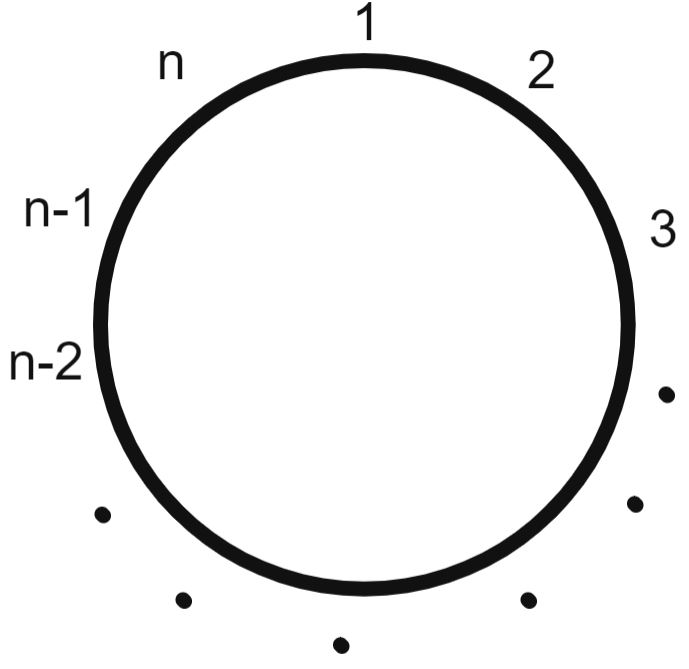
\includegraphics[width=\linewidth]{sol3} %тут поменять имя пикчи
    \end{figure}
    \end{minipage}
\end{minipage}

\textbf{Дефолтные математические знаки и символы:}\\
$\geqslant$,
$\leqslant$,
$a^{b}$,
$x_{i}$,
$\sqrt{a}$,
$\frac{a}{b}$,
$\displaystyle \frac{a}{b}$,
$\cdot$
$\;\Rightarrow\;$,
$\;\Leftrightarrow\;$,
$1{,}2$.
О промежутках:
$a\!b$,
$a\,b$,
$a\:b$,
$a\;b$,
$a\quad b$.

\textbf{Стандартные система и совокупность уравнений / неравенств:}\\
$\left\{
\begin{aligned}
f(x) &= 0 \\
g(x) &= 1
\end{aligned}\right.$

$\left[\begin{aligned}
&\left\{\begin{aligned}
f(x) &\geqslant a \\
g(x) &= b
\end{aligned}\right.\\
&\left\{\begin{aligned}
f(x) &< a \\
g(x) &= -b
\end{aligned}\right.
\end{aligned}\right.$

\subsection*{\textcolor{Emerald}{\textbf{Не математическое, но полезное:}}}
% комментарий в любом месте документа, который нигде не будет видно. Можно использовать для написания заметок-вопросов по задачам
\textbf{Пример таблицы:}

\begin{tabular}{|c|c|c|}
\hline
    $a$ & $b$ & текст
\\\hline
    $c$ & $d$ & мораль
\\\hline
\end{tabular}\\

\textbf{Отступы:} между\smallskip\\ строками\medskip\\ \textbf{Тире} --- это три дефиса.\\
\textbf{Списки:}
\begin{mylist}
\item [$\bullet$] это был пункт а
\item [2)] а это уже пункт номер 2 с изменённым заголовком
\end{mylist}

\subsection*{\textcolor{Emerald}{\textbf{Всё, неупомянутое выше (или если просто что-то не так):}}}
\begin{mylist}
\item [$\bullet$] Решение отдельных вопросов касательно ТеХа нужно искать в \href{https://www.mccme.ru/free-books/llang/newllang.pdf}{Львовском}.

\item [$\bullet$] Найти произвольный символ, который нужен, можно в \href{http://detexify.kirelabs.org/classify.html}{Detexify}.

\item [$\bullet$] Если возникли сомнения при решении, ответ практически ко всем задачам можно проверить с помощью \href{https://www.wolframalpha.com/}{WolframAlpha}.

\item [$\bullet$] Если в задаче нужно создать картинку, то лучше пока отложить эту задачу. Все графики планируется централизованно нарисовать (или перерисовать) в геогебре.

\item [\textcolor{brown}{\textbf{!!}}] Важно ставить \textcolor{red}{\textbf{$\spadesuit$}}
(или просто red) в тело задачи в случае серьёзных вопросов к решению и какой-то вопиющей лажи.

\item [\textcolor{brown}{\textbf{!!}}] Важно ставить \textcolor{olive}{\textbf{$\spadesuit$}}
(или просто olive) в тело задачи в случае не самого удачного текста и кривых отступов.
\end{mylist}

\subsection*{\textcolor{Violet}{\textbf{Комментарии:}}}% а также невидимые комментарии - так можно оставлять заметки-вопросы прямо в задаче, чтобы потом было понятно, в чём вопрос.
\begin{mylist}
\item [$\skull$] Переставлять задачи местами --- очень плохая идея.

\item [$\smiley$] При двойном клике по тексту pdf справа происходит автоматический переход к этому месту в латех-коде, а для обратного перехода можно нажать стрелку вправо (висит сверху между pdf и латех-кодом).

\item [$\smiley$] Если есть размышления, дописывать red/olive к задаче или не дописывать, то лучше всё-таки дописать.

\item [$\skull$] Самое плохое, что можно сделать --- написать в любое поле из трёх (НаписанноеРешение/ВерныйОтвет/Подсказка) только половину того, что надо, никак это не отметить, и потом пойти дальше.\\ Нужно в этот момент писать red/olive в случайном месте задачи, чтобы потом вычислить это с помощью Ctrl+F по всему документу (и это то, что потом будет делаться долго и тщательно)
\end{mylist}

\newpage
\setcounter{num}{627}

\hypertarget{7.6}{{\centering\section*{\bigskip\\\textcolor{Blue}{\hyperlink{start2}{\textcolor{Blue}{7.6}} Разложение на множители.}\vspace{-5mm}}}}

\begin{problem}{Вынесение общего множителя за скобки.}{7.6.2}{7A}{(лёгкая)}
{Решить уравнение: \\ $(x^{2} - 1)(x + 3)(x - 2) - (1 - x^{2})(2 - x)(2x + 2) - (x^{2} - 1)(x - 3)(2 - x) = 0$.}
{НаписанноеРешение}
{ВерныйОтвет}{Подсказка}
\end{problem}

\begin{problem}{Вынесение общего множителя за скобки.}{7.6.2}{7A}{(не лёгкая)}
{Найти корни уравнения: $(5x + 1)\cdot(x + 3) = (x + 4)\cdot\left(x + \frac{1}{5}\right)$.}
{Нетрудно заметить, что в нашем уравнении два множителя, а именно $5x + 1$ и $x + \frac15$, весьма похожи. В самом деле: $5x + 1 = 5\cdot(x + \frac15)$. Перенесём всё в левую часть уравнения и учтём этот факт: $(5x + 1)\cdot(x + 3) = (x + 4)\cdot\left(x + \frac{1}{5}\right) \;\Rightarrow\; $\smallskip\\
$(5x + 1)\cdot(x + 3) - (x + 4)\cdot\left(x + \frac{1}{5}\right) = 0 \;\Rightarrow\; 5\cdot\left(x + \frac{1}{5}\right)\cdot(x + 3) - (x + 4)\cdot\left(x + \frac{1}{5}\right) = 0$\smallskip\\
$\Rightarrow\; \left(x + \frac{1}{5}\right)\cdot(5(x+3) - (x+4)) = (x + \frac{1}{5})\cdot(4x + 11) = 0$.\smallskip\\
Произведение двух величин может быть равно нулю только в том случае, если хотя бы одна из этих величин равна нулю.\\
1) $x + \frac15 = 0 \;\Rightarrow\; x = -\frac15 = -0{,}2$.\\
2) $4x + 11 = 0 \;\Rightarrow\; 4x = -11 \;\Rightarrow\; x = -\frac{11}{4} = -2{,}75$.\\
Таким образом, данное уравнение имеет два решения: $x = -2{,}75$ и $x = -0{,}2$.}
{Корнями данного уравнения являются $x = -2{,}75$ и $x = -0{,}2$.}{Перенеси всё в одну часть уравнения и выдели общий множитель: для этого необходимо заметить, что два множителя тут похожи друг на друга.}
\end{problem}

\begin{problem}{Вынесение общего множителя за скобки.}{7.6.2}{7A}{(лёгкая)}
{Решить уравнение: $(3a - 7)(2a - 1)(7a - 5) = (14 - 6a)(3 - 6a)(5a - 7)$.}
{НаписанноеРешение}
{ВерныйОтвет}{Подсказка}
\end{problem}

\begin{problem}{Вынесение общего множителя за скобки.}{7.6.2}{7A}{(лёгкая)}
{Решить уравнение: $(x + 7)^{3} = 49(x + 7)$.}
{Поскольку обе части уравнения весьма похожи (и там, и там есть множитель $(x + 7)$), используем метод группировки: $(x + 7)^{3} = 49(x + 7) \;\Rightarrow\; (x + 7)^{3} - 49(x + 7) = 0 \;\Rightarrow\; (x + 7)((x + 7)^2 - 49) = 0$. Теперь можно преобразовать второй множитель: тут несложно заметить формулу разности квадратов, поэтому $(x + 7)((x + 7)^2 - 49) = 0 \;\Rightarrow\; (x + 7)(x + 7 - 7)(x + 7 + 7) = x(x + 7)(x + 14) = 0$.\\
Произведение нескольких чисел равно 0 в том и только в том случае, если какое-то из этих чисел равно 0. $\;x = 0$, $\;x + 7 = 0 \;\Rightarrow\; x = -7$, $\;x + 14 = 0 \;\Rightarrow\; x = -14$.\\
Итого, уравнение $(x + 7)^{3} = 49(x + 7)$ имеет три решения: $x = -14$, $x = -7$, $x = 0$.}
{Кубическое уравнение имеет три решения: $x = -14$, $x = -7$, $x = 0$.}{Перенеси всё в левую часть и используй метод группировки.}
\end{problem}

\begin{problem}{Вынесение общего множителя за скобки.}{7.6.2}{7A}{(лёгкая)}
{Найти все значения $x$, при которых уравнение $(4x - 2)(5x + 0{,}5) = -(1 - 2x)(10x + 1)$ будет верным.}
{НаписанноеРешение}
{ВерныйОтвет}{Подсказка}
\end{problem}

\begin{problem}{Метод группировки.}{7.6.3}{6K}{(лёгкая)}
{Разложить на множители-скобки: $\lambda\alpha - 5\lambda + 2\alpha - 10$.}
{НаписанноеРешение}
{ВерныйОтвет}{Подсказка}
\end{problem}

\begin{problem}{Разложение на множители с помощью ФСУ.}{7.6.4}{7A}{(лёгкая)}
{Вычислить значение выражения $a^{2} + b^{2} - 2ab$ при $a = \sqrt{3} - \sqrt{2} + 4$, $b = \sqrt{3} - \sqrt{2} + 6$.

}
{НаписанноеРешение}
{ВерныйОтвет}{Подсказка}
\end{problem}

\begin{problem}{Разложение на множители с помощью ФСУ.}{7.6.4}{7A}{*}
{Загадай произвольное нечётное целое число, вычисли его квадрат и вычти 1.\\ Утверждается, что полученное число всегда делится на 8.\\ Доказать это утверждение.}
{НаписанноеРешение}
{ВерныйОтвет}{Подсказка}
\end{problem}

\begin{problem}{Разложение на множители с помощью ФСУ.}{7.6.4}{6K}{(лёгкая)}
{Какое из данных выражений является квадратом двучлена (то есть, $(P + Q)^{2}$)?
\smallskip\\a) $a^{2} + 4b^{2}$; \hfill b) $a^{2} - 4b^{2}$; \hfill c) $a^{2} + 4b^{2} + 2ab$; \hfill d) $a^{2} + 4b^{2} - 4ab$.}
{Верный ответ~--- d): $\,a^{2} + 4b^{2} - 4ab = a^{2} - 4ab + 4b^{2} = (a - 2b)^2$.\\ Всё остальное не является нужной нам формулой сокращённого умножения (квадратом суммы) и потому не подходит.}
{Квадратом двучлена является выражение $a^{2} + 4b^{2} - 4ab$.}{Какое из этих выражений является нужной формулой сокращённого умножения (квадратом суммы)?}
\end{problem}

\begin{problem}{Разложение на множители с помощью ФСУ.}{7.6.4}{6K}{(лёгкая)}
{Найти одночлен, которым можно заменить $*$ в выражении $16m^{2} + 24mn + {*}$, \\чтобы полученный трёхчлен было бы можно представить как квадрат двучлена \\(то есть, $(A + B)^{2}$):
\smallskip\\а) $3n$; \hfill b) $3n^{2}$; \hfill c) $9n^{2}$; \hfill d) $9n$.}
{НаписанноеРешение}
{ВерныйОтвет}{Подсказка}
\end{problem}

\begin{problem}{Разложение на множители с помощью ФСУ.}{7.6.4}{6K}{(лёгкая)}
{Превратить в произведение многочлен $b^{2} - 4b + 4$.}
{Заметим, что данный многочлен похож на формулу сокращенного умножения: действительно, $b^2 = b\cdot b$, $\,4 = 2\cdot 2$, $\,-4b = -2\cdot2\cdot b$. То есть, перед нами квадрат разности, и $b^{2} - 4b + 4 = (b - 2)^2$. А это как раз произведение.

}
{$b^{2} - 4b + 4 = (b - 2)^2$.}{Тут можно заметить формулу сокращенного умножения.}
\end{problem}

\begin{problem}{Разложение на множители с помощью ФСУ.}{7.6.4}{6K}{(лёгкая)}
{Воспользоваться одной из формул сокращённого умножения и переписать\\ многочлен $c^{2} + 2c + 1$ в виде произведения.}
{Данное выражение похоже на формулу квадрата суммы $(A + B)^2 = \\ = A^2 + 2AB + B^2$. Понятно, что в нашем случае $A = c$, а $B = 1$.\\ Таким образом, $c^{2} + 2c + 1 = c \cdot c + 2 \cdot c  \cdot 1 + 1 \cdot 1 = (c + 1)^2$.}
{$c^{2} + 2c + 1 = (c + 1)^2$.}{Это квадрат суммы.}
\end{problem}

\begin{problem}{Разложение на множители с помощью ФСУ.}{7.6.4}{6K}{(лёгкая)}
{Воспользоваться одной из формул сокращённого умножения и переписать\\ многочлен $x^{2} + 4x + 4$ в виде произведения.}
{Данное выражение похоже на формулу квадрата суммы $(A + B)^2 = \\ = A^2 + 2AB + B^2$. В нашем случае $A = x$, а $B = 2$ (так как $2^2 = 4$ и $2 \cdot 2 = 4$).\\ Таким образом, $x^{2} + 4x + 4 = x \cdot x + 2 \cdot x \cdot 2 + 2 \cdot 2 = (x + 2)^2$.}
{$x^{2} + 4x + 4 = (x + 2)^2$.}{Это квадрат суммы.}
\end{problem}

\begin{problem}{Разложение на множители с помощью ФСУ.}{7.6.4}{6K}{(лёгкая)}
{Воспользоваться одной из формул сокращённого умножения и переписать\\ многочлен $s^{2} - 6s + 9$ в виде произведения.}
{Данное выражение похоже на формулу квадрата разности $(A - B)^2 = \\ = A^2 - 2AB + B^2$. В нашем случае $A = s$, а $B = 3$ (так как $3^2 = 9$ и $2 \cdot 3 = 6$).\\ Таким образом, $s^{2} - 6s + 9 = s \cdot s - 2 \cdot s \cdot 3 + 3 \cdot 3 = (s - 3)^2$.}
{$s^{2} - 6s + 9 = (s - 3)^2$.}{Это квадрат разности.}
\end{problem}

\begin{problem}{Разложение на множители с помощью ФСУ.}{7.6.4}{6K}{(лёгкая)}
{Воспользоваться одной из формул сокращённого умножения и переписать\\ многочлен $4a^{2} - 25$ в виде произведения.}
{Данное выражение похоже на формулу разности квадратов $A^2 - B^2 = \\ = (A - B)(A + B)$. В нашем случае можно догадаться, что $A = 2a$, а $B = 5$ (так как $2a \cdot 2a = 4a^2$ и $5^2 = 3$). Таким образом, $4a^{2} - 25 = 2a \cdot 2a - 5 \cdot 5 = (2a - 5)(2a + 5)$.

}
{$4a^{2} - 25 = (2a - 5) \cdot (2a + 5)$.}{Это разность квадратов.}
\end{problem}

\begin{problem}{Разложение на множители с помощью ФСУ.}{7.6.4}{6K}{*}
{Воспользоваться одной из формул сокращённого умножения и переписать\\ многочлен $9d^{2} + 12d + 4$ в виде произведения.}
{Это выражение похоже на формулу квадрата суммы, $A^2 + 2AB + B^2 = (A + B)^2$. $9d^2 = (3d)^2$, $4 = 2^2$, $12d = 2\cdot3d\cdot2$. Поэтому данное выражение представляет собой квадрат суммы, и $9d^{2} + 12d + 4 = (3d + 2)^2$.}
{$9d^{2} + 12d + 4 = (3d + 2)^2$.}{Это квадрат суммы.}
\end{problem}

\begin{problem}{Разложение на множители с помощью ФСУ.}{7.6.4}{6K}{*}
{Воспользоваться одной из формул сокращённого умножения и переписать\\ многочлен $\frac{1}{4}z^{2} - 4$ в виде произведения.}
{Данное выражение похоже на формулу разности квадратов $A^2 - B^2 = \\ = (A - B)(A + B)$. Немного подумав, можно понять, что $A = \frac12 z$, а $B = 2$ (так как $\frac12 z \cdot \frac12 z = \frac14 z^2$ и $2^2 = 4$). Таким образом, $\frac{1}{4}z^{2} - 4 = \frac12 z \cdot \frac12 z - 2 \cdot 2 = \left(\frac12 z - 2\right)\left(\frac12 z + 2\right)$.

}
{$\frac{1}{4}z^{2} - 4 = \left(\frac12 z - 2\right)\left(\frac12 z + 2\right)$.}{Это разность квадратов.}
\end{problem}

\begin{problem}{Разложение на множители с помощью ФСУ.}{7.6.4}{6K}{*}
{Воспользоваться одной из формул сокращённого умножения и найти значение выражения: $(a + 8)^{2} - 2(a - 2) \cdot (a + 8) + (a - 2)^{2}$.}
{Посмотрим на это выражение внимательно: тут есть квадрат выражения $a + 8$, квадрат выражения $a - 2$, и смешанное произведение, поэтому это должно быть квадратом разности. Применяем формулу $(A - B)^2 = A^2 - 2AB + B^2$ c $A = (a + 8)$ и $B = (a - 2)$. Получаем, что $(a + 8)^{2} - 2(a - 2) \cdot (a + 8) + (a - 2)^{2} = \\ = ((a + 8) - (a - 2))^2 = (a + 8 - a + 2)^2 = 10^2 = 100$.}
{После упрощения получается, что данное выражение равно 100.\\ Причём при любых значениях $a$ --- оно на самом деле от $a$ вообще не зависит.}{Тут можно заметить квадрат разности.}
\end{problem}

\begin{problem}{Разложение на множители с помощью ФСУ.}{7.6.4}{6K}{*}
{Воспользоваться одной из формул сокращённого умножения и найти значение выражения: $\,(4z^{2} + 3)^{2} + 2(4z^{2} + 3)(9 - 4z^{2}) + (4z^{2} - 9)^{2}$.}
{После некоторых размышлений становится заметно, что данное выражение похоже на квадрат суммы или разности, и в итоге это оказывается квадратом разности. Действительно: $\,(4z^{2} + 3)^{2} + 2(4z^{2} + 3)(9 - 4z^{2}) + (4z^{2} - 9)^{2} = (4z^{2} + 3)^{2} - 2(4z^{2} + 3)(4z^{2} - 9) + (4z^{2} - 9)^{2} = A^2 - 2AB + B^2$, где $A = 4z^2 + 3$, $B = 4z^2 - 9$. Получаем, что $(4z^{2} + 3)^{2} - 2(4z^{2} + 3)(4z^{2} - 9) + (4z^{2} - 9)^{2} = ((4z^2 + 3) - (4z^2 - 9))^2 = (4z^2 + 3 - 4z^2 + 9)^2 = 12^2 = 144$.}
{$(4z^{2} + 3)^{2} + 2(4z^{2} + 3)(9 - 4z^{2}) + (4z^{2} - 9)^{2} = 144$.}{Можно заметить, что это квадрат разности (или суммы).}
\end{problem}

\begin{problem}{Разложение на множители с помощью ФСУ.}{7.6.4}{6K}{(лёгкая)}
{Разложить на множители: $5t^{3} - 5k^{2}t$.}
{Понятно, что можно отделить множитель $5t$: $\;5t^{3} - 5k^{2}t = 5t \cdot (t^2 - k^2)$. Теперь используем формулу разности квадратов: $5t \cdot (t^2 - k^2) = 5t \cdot (t - k) \cdot (t + k)$. Выражение разложено на множители, дальше раскладывать некуда.}
{$5t^{3} - 5k^{2}t = 5t \cdot (t - k) \cdot (t + k)$.}{Вынеси множитель и используй формулу сокращённого умножения.}
\end{problem}

\begin{problem}{Разложение на множители с помощью ФСУ.}{7.6.4}{6K}{(лёгкая)}
{Разложить на множители выражение $-12x^{3} + 12x^{2} - 3x$.}
{Для начала, нетрудно заметить, что можно вынести множители 3, $x$, и $-1$: $\;-12x^{3} + 12x^{2} - 3x = 3x\cdot(-4x^2 + 4x - 1) = -3x \cdot (4x^2 - 4x + 1)$.\\ Теперь нетрудно заметить формулу сокращённого умножения: ведь выражение в скобках --- квадрат разности, и $-3x \cdot (4x^2 - 4x + 1) = -3x \cdot (2x - 1)^2$.}
{$-12x^{3} + 12x^{2} - 3x = -3x \cdot (2x - 1)^2$.}{Помимо всех множителей, ещё нужно заметить, что можно вынести множитель $-1$, а потом использовать формулу сокращённого умножения.}
\end{problem}

\begin{problem}{Разложение на множители с помощью ФСУ.}{7.6.4}{7A}{(лёгкая)}
{Разложить на множители: $(a - c)(a + c) + (a - b)^{2} - (a - b - c)(a - b + c) - 4$.}
{НаписанноеРешение}
{ВерныйОтвет}{Подсказка}
\end{problem}

\begin{problem}{Разложение на множители с помощью ФСУ.}{7.6.4}{7A}{(лёгкая)}
{Найти значение выражения $\sqrt{137^{2} - 88^{2}}$.}
{НаписанноеРешение}
{ВерныйОтвет}{Подсказка}
\end{problem}

\begin{problem}{Разложение на множители с помощью ФСУ.}{7.6.4}{9D}{*}
{Вычислить: $\sqrt{2160^{2} - 1296^{2}}$.}
{НаписанноеРешение}
{ВерныйОтвет}{Подсказка}
\end{problem}

\begin{problem}{Разложение на множители с помощью ФСУ.}{7.6.4}{6K}{*}
{Решить уравнение $9c^{2} - 16 = 0$.}
{Заметим, что данное выражение --- разность квадратов: получаем, что $9c^{2} - 16 = (3c - 4)(3c + 4) = 0$. Произведение двух чисел может быть равно нулю в том и только в том случае, если какое-то из этих чисел (или оба) равны нулю.\\
Значит, $3c - 4 = 0 \Leftrightarrow c = \frac43\,$ или $\,3c + 4 = 0 \Leftrightarrow c = -\frac43$.\\ Несложно убедиться, что оба числа являются корнями уравнения, так как при подстановке получается верное равенство $16 - 16 = 0$. Таким образом, $c = \pm\frac43$.}
{Уравнение $9c^{2} - 16 = 0$ имеет два корня: $c = \frac43\,$ и $\,c = -\frac43$.}{Выражение слева --- разность квадратов.\\
Когда произведение двух чисел равно нулю?}
\end{problem}

\begin{problem}{Разложение на множители с помощью ФСУ.}{7.6.4}{6K}{*}
{Решить уравнение $y^{2} + y = 0$.}
{Используем метод группировки, чтобы разложить данный двучлен на множители: $y^2 + y = y(y + 1)$. В итоге приходим к уравнению $y(y + 1) = 0$.\\ Произведение двух чисел может быть равно нулю в том и только в том случае, если какое-то из этих чисел (или оба) равны нулю.\\
Значит, $y = 0$ или $y + 1 = 0 \Leftrightarrow y = -1$. Несложно убедиться, что оба числа являются корнями уравнения: при подстановке $y = 0$ получаем верное равенство $0 + 0 = 0$, а при $y = -1$ получаем равенство $1 + (-1) = 0$.}
{Уравнение $y^{2} + y = 0$ имеет два корня: $y = 0$ и $y = -1$.}{Выражение слева нужно разложить на множители.}
\end{problem}

\begin{problem}{Разложение на множители с помощью ФСУ.}{7.6.4}{6K}{(лёгкая)}
{Решить уравнение $t(t + 1)(t - 2)(t^2 + 1) = 0$.}
{Произведение нескольких чисел может быть равно нулю в том и только в том случае, когда какое-то из этих чисел равно нулю. Если $t = 0$, то $0$ --- корень данного уравнения. Если $t + 1 = 0$, то $t = -1$ является корнем. Если $t - 2 = 0$, то $t = 2$ --- корень. $t^2 + 1$ --- это сумма положительных чисел, поэтому она никогда не равна 0. Итого, мы нашли 3 решения: $t = -1$, $t = 0$, и $t = 2$.}
{Данное уравнение имеет три решения: $t = -1$, $t = 0$, и $t = 2$.}{Когда произведение нескольких чисел может быть равно нулю?}
\end{problem}

\begin{problem}{Разложение на множители с помощью ФСУ.}{7.6.4}{6K}{*}
{Решить уравнение $d^{2} - 8d + 16 = 9$.}
{Заметим, что левая часть уравнения является формулой сокращённого умножения: это квадрат разности $(A - B)^2 = A^2 - 2AB + B^2\,$ с $A = d$, $B = 4$.\\ Поэтому $(d - 4)^2 = 9$, или, что то же самое, $(d - 4)^2 = 3^2$.\\ Поскольку <<минус на минус даёт плюс>>, возможны два варианта:\\
Вариант №1: $\;d - 4 = 3 \;\Rightarrow\; d = 7$.\hfill Вариант №2: $\;d - 4 = -3 \;\Rightarrow\; d = 1$.\smallskip\\
Проверка: $d = 7 \;\Rightarrow\; 49 - 56 + 16 = 9$ \hfill $d = 1 \;\Rightarrow\; 1 - 8 + 16 = 9$.}
{Уравнение имеет два решения: $d = 1$ и $d = 7$.}{Выражение слева~--- квадрат разности.}
\end{problem}

\begin{problem}{Разложение на множители с помощью ФСУ.}{7.6.4}{6K}{*}
{Решить уравнение: $\lambda^{2} - 4\lambda - 21 = 0$.}
{Искусственно соберём в левой части уравнения формулу сокращённого умножения (квадрата разности). $(A - B)^2 = A^2 - 2AB + B^2$.\\ У нас $A = \lambda$, поэтому $2AB = 2\lambda \cdot B = 4\lambda \;\Rightarrow\; B = 2$. Для формулы сокращённого умножения не хватает $B^2$, то есть $2^2 = 4$. Сделаем так: $\lambda^{2} - 4\lambda - 21 = 0 \;\Rightarrow\; \lambda^{2} - 4\lambda = 21 \;\Rightarrow\; \lambda^{2} - 4\lambda + 4 = 21 + 4 \;\Rightarrow\; (\lambda - 2)^2 = 25$.\\ Тогда под квадратом должно быть либо $5$, либо $-5$:\\ $\lambda - 2 = 5 \;\Rightarrow\; \lambda = 7$.\hfill $\lambda - 2 = -5 \;\Rightarrow\; \lambda = -3$.\smallskip\\ Оба решения, как показывает проверка, подходят:\\ $7\cdot7 - 4\cdot7 - 21 = 49 - 28 - 21 = 0$,\hfill $(-3)\cdot(-3) - 4\cdot(-3) - 21 = 9 + 12 - 21 = 0$.}
{Квадратное уравнение имеет два решения: $\lambda = -3$ и $\lambda = 7$.}{После небольшого добавления к обеим частям уравнения, в левой части уравнения можно соорудить квадрат разности, а затем решить полученное уравнение также, как и уравнение $p^2 = q^2$.}
\end{problem}

\begin{problem}{Разложение на множители с помощью ФСУ.}{7.6.4}{6K}{*}
{Решить уравнение: $a^{2} - 2a = 80$.}
{НаписанноеРешение}
{ВерныйОтвет}{Подсказка}
\end{problem}

\begin{problem}{Разложение на множители с помощью ФСУ.}{7.6.4}{6K}{*}
{Решить уравнение: $b^{2} + 2b = 99$.}
{НаписанноеРешение}
{ВерныйОтвет}{Подсказка}
\end{problem}

\begin{problem}{Разложение на множители с помощью ФСУ.}{7.6.4}{6K}{*}
{Решить уравнение: $c^{2} - 4c - 45 = 0$.}
{Заметим, что в этом выражении почти собирается формула сокращённого умножения: $c \cdot c = c^2$ присутствует, $2\cdot c \cdot \textcolor{Emerald}{2}$ на месте, не хватает только $\textcolor{Emerald}{2}^2 = 4$. Используем хитрость: $c^{2} - 4c - 45 = 0 \;\Rightarrow\; c^2 - 4c + 4 - 4 - 45 = 0 \;\Rightarrow\; (c^2 - 4c + 4) - 49 = 0 \;\Rightarrow\; (c - 2)^2 - 7^2 = 0$. Можно продолжить дальше: теперь мы видим формулу разности квадратов $A^2 - B^2 = (A - B)(A + B)$ с $A = c - 2$, $B = 7$. Получаем, что $(c - 2)^2 - 7^2 = (c - 2 - 7)\cdot(c - 2 + 7) = (c - 9)\cdot(c + 5) = 0$.\smallskip\\
Произведение двух чисел равно нулю в том и только в том случае, если одно из этих чисел равно 0. А значит, или $c - 9 = 0$, и тогда $c = 9$, или $c + 5 = 0$, и $c = -5$.\smallskip\\
Таким образом, мы нашли целых два решения у уравнения: это $c = -5$ и $c = 9$.}
{Уравнение $c^{2} - 4c - 45 = 0$ имеет два решения: $c = -5$ и $c = 9$.}{Прибавь и вычти 4, для того чтобы одновременно и не изменить уравнение, и получить некоторую формулу сокращённого умножения.\\
После этого должна получиться разность квадратов (и нужно опять использовать формулу сокращённого умножения). Когда произведение двух чисел равно 0?}
\end{problem}

\begin{problem}{Разложение на множители с помощью ФСУ.}{7.6.4}{6K}{*}
{Решить уравнение: $d^{2} + 6d = 55$.}
{Нам было бы гораздо проще решить это уравнение, если бы оно имело вид $x^2 = 8^2$. Чтобы упростить наше уравнение, выделим в этом выражении полный квадрат. Для этого используем хитрость: $d^2 + 6d = 55 \;\Rightarrow\; d^2 + 6d + 9 = 55 + 9 \;\Rightarrow\; (d + 3)^2 = 64 \;\Rightarrow\; (d + 3)^2 - 8^2 = 0$.\\ Теперь выражение слева --- это разность квадратов, и мы можем использовать известную нам формулу разности квадратов с $A = d + 3$, $B = 8$.\\ Получаем, что $(d + 3 - 8)\cdot(d + 3 + 8) = (d - 5)\cdot(d + 11) = 0$.\\
Произведение двух чисел равно нулю в том и только в том случае, если одно из этих чисел равно нулю. То есть $d - 5 = 0 \;\Leftrightarrow\; d = 5$ или $d + 11 = 0 \;\Leftrightarrow\; d = -11$.\smallskip\\ Таким образом, мы нашли целых два решения у уравнения: это $d = -11$ и $d = 5$.}
{Уравнение $d^{2} + 6d = 55$ имеет два решения: $d = -11$ и $d = 5$.}{Прибавь к обеим частям уравнения такое число, чтобы получить формулу сокращённого умножения. После этого получи в одной части уравнения разность квадратов и используй формулу, чтобы разложить выражение на множители. Когда произведение двух чисел равно 0?}
\end{problem}

\begin{problem}{Разложение на множители с помощью ФСУ.}{7.6.4}{6K}{*}
{Решить уравнение: $e^{2} + 10e = -24$.}
{Данное уравнение было бы гораздо проще решить, если бы оно имело вид $A^2 = B^2$. Поэтому нам нужно каким-то образом выделить полный квадрат, для этого надо превратить это выражение в квадрат суммы: $e^2 + 10e = -24 \;\Rightarrow\; e^2 + 10e + 24 = 0 \;\Rightarrow\; e^2 + 10e + 24 + 1 = 1 \;\Rightarrow\; e^2 + 10e + 25 = 1 \;\Rightarrow\; (e + 5)^2 = 1$.\\
Далее, $(e + 5)^2 = 1 \;\Rightarrow\; (e + 5)^2 - 1 = 0 \;\Rightarrow\; (e + 5 - 1)(e + 5 + 1) = (e + 4)(e + 6) = 0$ (была использована формула для разности квадратов).\\
Произведение двух чисел равно 0 в том и только в том случае, если какое-то из этих чисел равно 0. $\;e + 4 = 0 \;\Rightarrow\; e = -4$, $\;e + 6 = 0 \;\Rightarrow\; e = -6$.}
{Данное квадратное уравнение имеет два решения, $e = -6$ и $e = -4$.}{Нужно модифицировать уравнение (оставляя его верным), выделить квадрат суммы, и свести уравнение к более простому уравнению $A^2 = B^2$.}
\end{problem}

\begin{problem}{Разложение на множители с помощью ФСУ.}{7.6.4}{6K}{*}
{Решить уравнение $f^{2} - 12f + 11 = 0$.}
{НаписанноеРешение}
{ВерныйОтвет}{Подсказка}
\end{problem}

\begin{problem}{Разложение на множители с помощью ФСУ.}{7.6.4}{6K}{*}
{Решить уравнение: $x^{2} - 14x + 38 = -2$.}
{Искусственно соберём в левой части уравнения формулу сокращённого умножения (квадрата разности). $(A - B)^2 = A^2 - 2AB + B^2$.\\ У нас $A = x$, поэтому $2AB = 2x \cdot B = 14x \;\Rightarrow\; B = 7$.\\ Для формулы сокращённого умножения не хватает $B^2$, то есть $7^2 = 49$.\\ Добавим ещё $11$ к обеим частям уравнения ($49 = 38 + 11$): $x^{2} - 14x + 38 = -2 \;\Rightarrow\; x^{2} - 14x + 38 + 11 = -2 + 11 \;\Rightarrow\; x^2 - 14x + 49 = 9 \;\Rightarrow\; (x - 7)^2 = 9$.\\ Тогда под квадратом должно быть либо $3$, либо $-3$:\\ $x - 7 = 3 \;\Rightarrow\; x = 10$.\hfill $x - 7 = -3 \;\Rightarrow\; x = 4$.\smallskip\\ Оба решения, как показывает проверка, подходят:\\ $10^2 - 14 \cdot 10 + 38 = 100 - 140 + 38 = -2$,\hfill $4^2 - 14 \cdot 4 + 38 = 16 - 56 + 38 = -2$.}
{Квадратное уравнение имеет два решения: $x = 4$ и $x = 10$.}{После небольшого добавления к обеим частям уравнения, в левой части уравнения можно соорудить квадрат разности, а затем решить полученное уравнение также, как и уравнение $p^2 = q^2$.}
\end{problem}

\begin{problem}{Комбинированные задачи.}{7.6.5}{7A red многопунктовая разбить на две}{(лёгкая)}
{Разложить на неразложимые множители (так, чтобы дальнейшее разложение было невозможным):\\
a) $x^{3} + 6x^{2} - 16x - 96$; \\b)* $9 + 25x^{2} - 16y^{2} - 30x$.}
{НаписанноеРешение}
{ВерныйОтвет}{Подсказка}
\end{problem}

\begin{problem}{Комбинированные задачи.}{7.6.5}{6K}{(лёгкая)}
{Решить уравнение $z^{2} + 3z + 3 = 9z - 6$.}
{Для упрощения перенесём всё в левую часть уравнения и приведём подобные члены: получаем, что $z^{2} + 3z + 3 - (9z - 6) = z^2 - 6z + 9 = 0$.\\
Однако, тут заметна формула сокращённого умножения: $z^2 - 6z + 9 = (z - 3)^2$. Таким образом, мы пришли к уравнению $(z - 3)^2 = 0$. Но если какое-то число в квадрате равно нулю, то это число --- ноль! Значит, $z - 3 = 0$, откуда $z = 3$.}
{Решением уравнения является $z = 3$.}{Нужно собрать всё в одной части уравнения и увидеть формулу сокращённого умножения.}
\end{problem}

\begin{problem}{Комбинированные задачи.}{7.6.5}{7A}{(лёгкая)}
{Решить уравнение: $x^{3} - x^{2} = 16x - 16$.}
{Разложим на множители выражения в обеих частях уравнения: \\$x^{3} - x^{2} = 16x - 16 \;\Rightarrow\; x^2(x - 1) = 16(x - 1)$. Видно, что у этих выражений есть общий множитель $x - 1$. Для того, чтобы провести группировку, перенесём всё в левую часть уравнения: $x^2(x - 1) - 16(x - 1) = 0 \;\Rightarrow\; (x^2 - 16)(x - 1) = 0$.\\ Используем формулу сокращённого умножения, так как первый множитель представляет собой разность квадратов: в итоге получаем, что $(x - 4)(x + 4)(x - 1) = 0$. Произведение нескольких множителей может быть равно 0 только тогда, когда один из этих множителей --- ноль. Получаем три разных варианта:\\
1) $x - 4 = 0 \;\Rightarrow\; x = 4; \qquad\;$
2) $x + 4 = 0 \;\Rightarrow\; x = -4; \qquad\;$
3) $x - 1 = 0 \;\Rightarrow\; x = 1$.\\
Все три числа --- $x = 4$, $x = -4$, $x = 1$ --- являются решениями этого уравнения.}
{Решениями этого уравнения являются числа $-4$, $1$, $4$.}{Разложи на множители, сгруппируй, используй формулу сокращённого умножения.}
\end{problem}

\begin{problem}{Комбинированные задачи.}{7.6.5}{6K}{(лёгкая)}
{С помощью метода группировки превратить многочлен $c^{3} + c^{2} - 3c - 3$ в произведение скобок.}
{Группируем слагаемые: $c^{3} + c^{2} - 3c - 3 = c^2(c + 1) - (3c + 3) = c^2(c + 1) - 3(c + 1) = (c^2 - 3)(c + 1) = (c - \sqrt{3})(c + \sqrt{3})(c + 1)$. Готово.}
{$c^{3} + c^{2} - 3c - 3 = (c - \sqrt{3})(c + \sqrt{3})(c + 1)$.}{После использования метода группировки можно дополнительно задействовать формулу разности квадратов.}
\end{problem}

\begin{problem}{Комбинированные задачи.}{7.6.5}{6K}{*}
{Показать, что выражение $x^{2} - 4x + 5$ принимает положительные значения при любых значениях $x$ (то есть, если для конкретного $x$ посчитать значение, всегда выйдет число, большее $0$).}
{НаписанноеРешение}
{ВерныйОтвет}{Подсказка}
\end{problem}

\begin{problem}{Комбинированные задачи.}{7.6.5}{7A}{*}
{Два различных вещественных числа $x$ и $y$ таковы, что $x^{2} + 2020y = y^{2} + 2020x$. Найти сумму чисел $x$ и $y$.}
{Поскольку нам неизвестно практически ничего, сделаем хоть что-то из того, что мы умеем: например, мы можем вынести общие множители: $x^{2} + 2020y = y^{2} + 2020x \;\Rightarrow\; x^2 - y^2 = 2020x - 2020y \;\Rightarrow\; (x - y)(x + y) = 2020(x - y)$, или $(x - y)(x + y - 2020) = 0$. Выглядит уже получше. Присмотримся повнимательнее: тут есть сумма чисел, $x + y$ --- её нам как раз и надо найти, и $x - y$, разность этих двух чисел. Мы точно знаем, что эти два числа различны, а значит $x - y \neq 0$.\smallskip\\
Получается, что $(x - y)(x + y - 2020) = 0 \;\Leftrightarrow\; x + y - 2020 = 0 \;\Leftrightarrow\; x + y = 2020$. То есть в любом случае сумма чисел равна 2020 --- иначе 0 не получится.}
{Сумма чисел $x$ и $y$ равна 2020.}{Перенеси всё в одну часть уравнения и разложи на множители.}
\end{problem}

\begin{problem}{Комбинированные задачи.}{7.6.5}{7A}{*}
{Найти $x^{3} + y^{3}$, если известно, что $x + y = 5$ и $x + y + x^{2}y + xy^{2} = 24$.}
{НаписанноеРешение}
{ВерныйОтвет}{Подсказка}
\end{problem}

\begin{problem}{Комбинированные задачи.}{7.6.5}{9I}{(лёгкая)}
{Вычислить значение выражения $\sqrt{28 - 6\sqrt{3}} - \sqrt{31 + 12\sqrt{3}}$.}
{НаписанноеРешение}
{ВерныйОтвет}{Подсказка}
\end{problem}

\begin{problem}{Тождества.}{7.6.6}{6K}{(лёгкая)}
{Найти среди указанных равенств тождество:
\\a) $\displaystyle a^{4} \cdot a^{5} = a^{20}$;
\\b) $\displaystyle a^{16} : a^{2} = a^{8}$;
\\c) $\displaystyle a^{6} b^{6} = \left(ab\right)^{12}$;
\\d) $\displaystyle \left(a^{3}\right)^{3} \cdot a^{3} = a^{12}$.}
{НаписанноеРешение}
{ВерныйОтвет}{Подсказка}
\end{problem}

\begin{problem}{Тождества.}{7.6.6}{7A}{(лёгкая)}
{(Тождество Диофанта) Показать, что $(a^{2} + b^{2})(c^{2} + d^{2}) = (ac + bd)^{2} + (ad - bc)^{2}$}
{НаписанноеРешение}
{ВерныйОтвет}{Подсказка}
\end{problem}

\begin{problem}{Тождества.}{7.6.6}{6K}{(лёгкая)}
{Указать многочлен, который тождественно равен многочлену (раскрыть скобки) $$(12xy - 2y^{2} + 6x^{2}) - (-3x^{2} - 2y^{2} + 8xy).$$ a) $3x^{2} + 20xy - 4y^{2}$; \hfill b) $9x^{2} + 4xy$; \hfill c) $9x^{2} + 20xy$; \hfill d) $3x^{2} + 4xy - 4y^{2}$.}
{Раскроем скобки: $(12xy - 2y^{2} + 6x^{2}) - (-3x^{2} - 2y^{2} + 8xy) = 12xy - 2y^2 + 6x^2 + 3x^2 + 2y^2 - 8xy = 4xy + 9x^2$ ($2y^2$ и $-2y^2$ сокращаются).\\
$4xy + 9x^2 = 9x^2 + 4xy$. Правильный ответ~--- b).}
{$9x^{2} + 4xy$, правильный ответ~--- b)}{Раскрыть скобки и привести подобные члены.}
\end{problem}

\begin{problem}{Тождества.}{7.6.6}{6K}{*}
{Чему равно значение выражения $3a^{2} - 12a - 3$, если $a^{2} - 4a + 2 = 6$?}
{НаписанноеРешение}
{ВерныйОтвет}{Подсказка}
\end{problem}

\end{document}